\chapter{Introduction}

start with neutrino prediction by pauli in beta decay, then talk about neutrinos and maybe even mention your dumb "extremes in experimental technique thing", but that's dumb as the main point.

And while the first indication of neutrinos came from the "missing" energy they took away from single beta decays, we now look for the mode of double beta decay which looks like single beta decay was expected to look -- where there are no neutrinos.  No, this is pretty dumb.

or:  we search for electrons coming out in double beta decay 

maybe here you should talk about neutrinos' aid in glimpsing certain things, like inner star workings and super novae, and at the beginnings of the universe

\section{Neutrinos}

Neutrinos are chargeless leptons which only interact via the weak force (and gravity).  There are three known ``flavors'' of neutrinos, each corresponding to one of the three known leptons:  $\nu_{e}$, $\nu_{\mu}$, and $\nu_{\tau}$.  These are the eigenstates in the basis of the weak force, so they are the states in which a neutrino will interact via the weak force.

{\color{gray}\emph{History:  }Neutrinos were first proposed while studying beta decay.  If the emitted electron and daughter nucleus in beta decay were the only products, the electron's energy should be essentially the same for every observed beta decay for a given isotope, since there is a certain energy difference between the initial and final states of the nucleus, and since the final kinetic energy of the nucleus is negligible due to its mass.  But instead of a sharp peak at this Q-value, a very broad electron energy spectrum is observed, all beneath and decreasing toward the Q-value.

In 1930, Wolfgang Pauli proposed that this variable ``loss'' in energy could be due to an additional particle being emitted along with the electron, but which is not observed.

[Fermi, massless]

[observation, and discovery of nu mu]}

\subsection{Neutrino Oscillation and Mass}

{\color{red}Neutrinos exhibit mixing between their energy eigenstates and their weak force eigenstates, and these are not the same basis. }  {\color{red}\textbf{not really:}  This means that a flavor eigenstate is not a stationary state} [the fact is that quark mixing happens, and one theory was that neutrinos would do something similar, and then oscillation is discovered...etc.]--- a neutrino which begins as a pure flavor state (as all neutrinos will, coming out of a quantum process involving one of the three leptons) will oscillate into the other two flavors as it evolves in time, i.e. the probability of measuring it to be one of the other two flavors is no longer zero.

{\color{gray}\emph{History:  }The first indications of neutrino oscillation came around 1970 with the Ray Davis Experiment [ref.], which measured the flux (at Earth) of solar electron neutrinos.  The flux measured was quite a bit lower than predicted by solar models, and this became known as the Solar Neutrino Problem.  The discovery of neutrino oscillation in the late 1990s [ref.] solved this problem, as only a fraction of the sun's neutrinos, produced as pure electron neutrinos, would interact as such.}

The very small mass of a neutrino, specifically relative to its momentum, lets one write its Hamiltonian in terms of mass squared differences $\Delta m_{ij}^{2} = m_{i}^{2} - m_{j}^{2}$, where $i$,$j$ = 1,2,3, referring to what we then call mass states.  The mass basis is really the energy basis with the small mass approximation, along with dropping some constant terms in the Hamiltonian (which do not affect time evolution).  Writing the time evolution in terms of mass squared differences means that neutrino oscillation experiments can produce measurements of these differences.  In fact, the discovery of neutrino oscillation was the first (and only, so far) demonstration that neutrinos have a non-zero mass.  Without neutrino mass (particularly without differences between the masses of the mass states), neutrinos would not oscillate.

Neutrino oscillation experiments also provide measurements on the amount of mixing between the flavor basis and the mass basis.  We define the mixing between them by a rotation in terms of three mixing angles, $\theta_{12}$, $\theta_{23}$, and $\theta_{13}$.  Transformation between the flavor and mass bases is done with the following unitary matrix, called the Pontecorvo--Maki-–Nakagawa–-Sakata (PMNS) matrix:

\begin{equation}
\begin{aligned}
U &= \begin{pmatrix}
1 & 0 & 0 \\
0 & c_{23} & s_{23} \\
0 & -s_{23} & c_{23} \end{pmatrix}
\begin{pmatrix}
c_{13} & 0 & s_{13} e^{-i \delta} \\
0 & 1 & 0 \\
-s_{13} e^{i \delta} & 0 & c_{13} \end{pmatrix}
\begin{pmatrix}
c_{12} & s_{12} & 0 \\
-s_{12} & c_{12} & 0 \\
0 & 0 & 1 \end{pmatrix}
\begin{pmatrix}
1 & 0 & 0 \\
0 & e^{i \alpha_{1}/2} & 0 \\
0 & 0 & e^{i \alpha_{2}/2} \end{pmatrix} \\
& = \begin{pmatrix}
c_{12} c_{13} & s_{12} c_{13} & s_{13} e^{-i \delta} \\
-s_{12} c_{23} - c_{12} s_{23} s_{13} e^{i \delta} & c_{12} c_{23} - s_{12} s_{23} s_{13} e^{i \delta} & s_{23} c_{13} \\
s_{12} s_{23} - c_{12} c_{23} s_{13} e^{i \delta} & -c_{12} s_{23} - s_{12} c_{23} s_{13} e^{i \delta} & c_{23} c_{13} \end{pmatrix}
\begin{pmatrix}
1 & 0 & 0 \\
0 & e^{i \alpha_{1}/2} & 0 \\
0 & 0 & e^{i \alpha_{2}/2} \end{pmatrix}
\end{aligned}
\label{eqn:umatrix}
\end{equation}

\noindent
where $c_{ij} = \cos \theta_{ij}$ and $s_{ij} = \sin \theta_{ij}$.  $\delta$ is a phase factor related to lepton CP violation, and $\alpha_{i}$ are Majorana phases.

Studying oscillations of neutrinos from different kinds of sources, with different energies and path lengths, can isolate sensitivities to the different parameters {\color{gray}(not really sure if this is the right thing to say)}.  For example, the study of solar neutrinos (neutrinos emanating from nuclear fusion reactions in the core of the sun) provides sensitivity to $\theta_{12}$ and $\Delta m_{12}^{2}$ {\color{gray}(\emph{right? $\theta_{12}$ may not be specifically solar...})}.  Beamline neutrino detectors can be designed for maximum sensitivity to parameters.  The parameters so far measured are as follows in Table  \ref{table:nu_osc_vals}:

\begin{table}[!htbp]
\caption{up to date values with references, and denote ``solar'', ``atmos.'', etc.} %not sure what [Small Table], between \caption and {}, w/ no spaces, does
\label{table:nu_osc_vals}
\begin{tabular}{c|c}
Parameter & Measurement \\
\hline
$\Delta m_{12}^{2}$ & \\
$|\Delta m_{31}^{2}|$ & \\
$\sin^{2} \theta_{12}$ & \\
$\sin^{2} \theta_{23}$ & \\
$\sin^{2} \theta_{13}$ & \\
\end{tabular}
\end{table}

Note that only the absolute value of $\Delta m_{31}^{2}$ is known.  As a consequence, there are two possibilities for the hierarchy of the three neutrino masses.  These are called the Normal and Inverted Hierarchies, as shown in Fig. \ref{fig:numasshier}.

\begin{figure}[H]
        \centering
                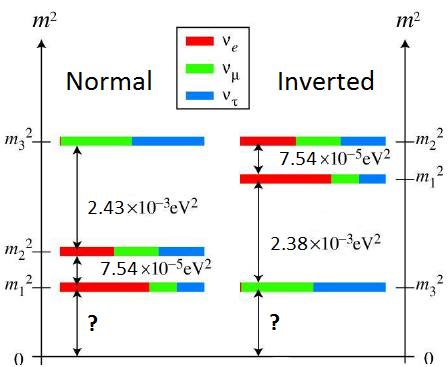
\includegraphics[width=.5\textwidth]{figures/hierarchy_alterred.png}
                \caption{The two possible hierarchies of neutrino masses.  The colors depict the mixing between the mass and flavor bases. {\color{red}\textbf{[ref]}}}
\label{fig:numasshier}
\end{figure}

\noindent
The correct mass hierarchy remains unknown, but next-generation neutrino experiments, possibly including nEXO, will be able to discern this.

Neutrino oscillation demonstrates that neutrinos have non-zero mass, and though oscillation experiments can measure the mass squared differences, we still do not have a measurement of the absolute masses of the three neutrinos.  {\color{gray}\emph{History:  }mention Pauli's first statement of limit near electron mass?  Then maybe say the 0 assumption, which I think came from Fermi's beta decay theory, but if you mention that above, just refer to it here.}

The current upper limits on the mass come from...(KATRIN(\rightarrow\nu_{e})?  Cosmology(\rightarrow sum)?

Neutrinoless double beta decay experiments like EXO-200 can put upper limits on specifically the Majorana neutrino mass (i.e., upper limits on the neutrino mass if neutrinos are indeed Majorana particles).  As discussed in the next chapter, [EXO-200 and KamLAND (sp?) ZEN (sp?) together provide the strongest Majorana neutrino mass upper limit of [] (IS THAT TRUE?)].

Neutrino oscillation and non-zero neutrino mass are physics beyond the Standard Model (SM) of particle physics, and though much has been discovered through oscillation experiments, there is much yet to learn about neutrinos. Since they are chargeless, they may be Majorana particles, and their small mass could be explained by the See-saw Mechanism [ref]. Majorana particles are their own anti-particle, and this, along with the discovery that neutrinos have mass, allows for a unique test of the Majorana (vs. Dirac) nature of neutrinos: neutrinoless double beta decay.

\subsection{Neutrinoless Double Beta Decay}

Double beta decay is the simultaneous emission of two electrons from a nucleus.  Two-neutrino double beta decay, shown in Fig. \ref{fig:feynman_diags}(left), is allowed by the Standard Model and has been observed in several isotopes which are listed in Table (table).  Similar to beta decay, a neutrino accompanies each electron in this decay, broadening the spectrum of the summed electron energy. This is a second-order process, making it a rare decay, and requiring low backgrounds to measure.

\begin{figure}[H]
        %\centering
        \begin{subfigure}
                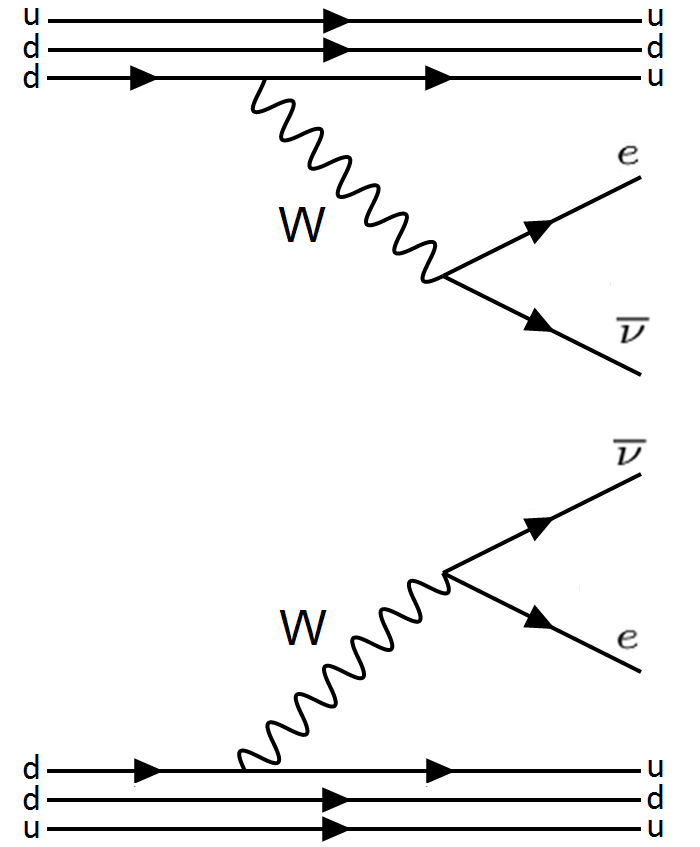
\includegraphics[width=.35\textwidth]{figures/feynman_2nu_quarks.png}
                %\caption{barf}
%        %\end{subfigure}
        %\begin{subfigure}
                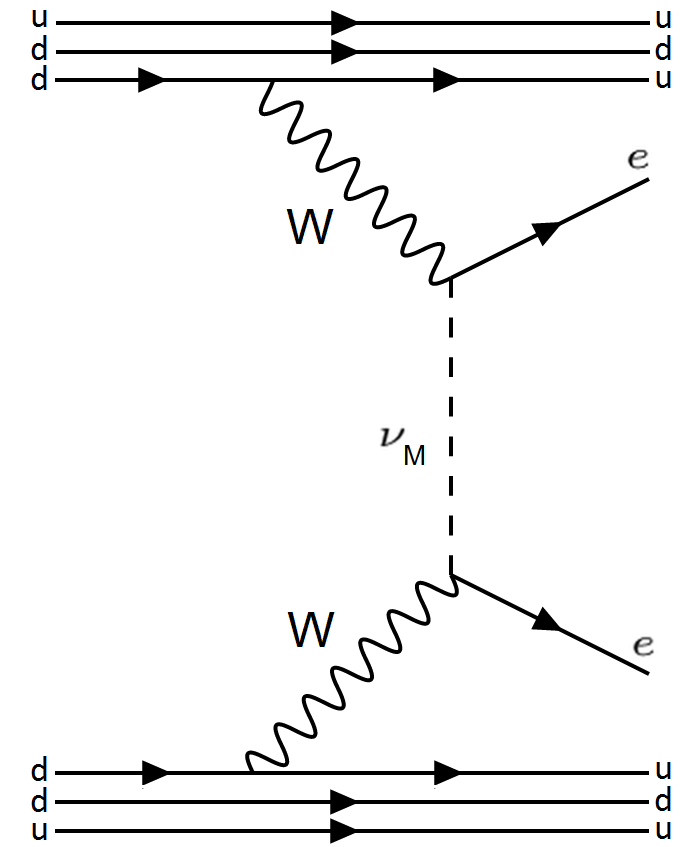
\includegraphics[width=.35\textwidth]{figures/feynman_0nu_quarks.png}
                \caption{Two-neutrino (left) and Neutrinoless (right) double beta decay.}
        \end{subfigure}
        \label{fig:feynman_diags}
\end{figure}

Neutrinoless double beta decay is a postulated mode of double beta decay, and is shown in Fig. \ref{fig:feynman_diags}(right). In this case, the neutrino is exchanged as a virtual particle (which would require that it is a Majorana particle), and there are no neutrinos in the final products. If discovered, not only would neutrinos be determined Majorana particles, but their absolute mass could also be measured in the form of an effective electron neutrino mass, since the rate of neutrinoless double beta decay will depend on the absolute neutrino mass as shown in Eqn. \ref{eqn:rate_vs_mass}:

\begin{equation}
T_{1/2}^{0\nu} = (G^{0\nu}(Q,Z)|M^{0\nu}|^{2}\braket{m_{\nu}}^{2})^{-1}
\label{eqn:rate_vs_mass}
\end{equation}

\noindent
where $T_{1/2}^{0\nu}$ is the $0\nu\beta\beta$ half-life,  $G^{0\nu}$ is a known phase space factor, and $M^{0\nu}$ is a model-dependent nuclear matrix element. The effective electron neutrino mass $\braket{m_{\nu}}$ is the expectation value of the mass for a pure electron neutrino:

\begin{equation}
\braket{m_{\nu}} = \sum\limits_{i} U_{ei}^{2} m_{i}.
\label{eqn:effectivemass}
\end{equation}

[how you detect it]
Two-neutrino gives broad while neutrinoless gives...
...delta function, just as expected for the single electron in beta decay before the discovery of the neutrino.

[experiments -- refer to next section for EXO]

\section{Enriched Xenon Observatory}

The Enriched Xenon Observatory (EXO) is a set of two experiments, each a LXe time projection chamber (TPC) designed to study the double beta decay of the isotope \textsuperscript{136}Xe, and ultimately to search for the zero-neutrino mode.  There are several advantages to a LXe detector.  Xe scintillates at [around?] [xxx] nm, which is [efficiently collected by [type that the APDs are]] [reference]; so the Xe acts as a detection medium in addition to being the source of the double beta decay [reference? I didn't make up that kind of sentence].  Xe can also be continuously purified to maintain large electron lifetimes in the LXe.  Also, the ratio between observed scintillation light and remaining ionized electrons (drifted from the decay site by the TPC's electric field) exhibits a well-known microscopic anti-correlation [ref.], the understanding of which improves the energy resolution of the detector.  Finally, a LXe TPC approach offers the opportunity, [fairly] unique in double beta decay, to "tag" the daughter, in this case Ba, at the site of the double beta decay event (specifically, of course, the neutrinoless ones).

EXO-200 is the first of the two experiments, and has been operational since April of 20[xx](?).  It is a liquid xenon TPC designed to probe Majorana neutrino masses down to around 100~meV.  [EXO instrum. paper part I]  The following sections decribe the EXO-200 experiment, as well as nEXO, the next-generation tonne-scale liquid xenon TPC which is now in the design stages.  EXO-200 does not have Ba tagging implemented, but it is hoped that nEXO will.

\subsection{EXO-200}



\subsection{nEXO}

\noindent
{\color{gray}\textbf{old stupid intro:}

The study of the neutrino has required extremes in experimental technique from the beginning.  Neutrinos were described by W. Pauli, who first proposed their existence to remedy an apparent violation of energy conservation in beta decay, as being [impossible to detect] [ref.].  Rather, it requires a great deal of sensitiviy, ingenuity, and hardship (just "ingenuity and hardship"?  sensitivity may be redundant) to observe them, and it was [] years before they were first observed by [Reines and Cowan] in [], by [] [ref.].  (is "rather, ..." too demoting-sounding?  it is absolutely not meant to be, of course)

Neutrino experiments of greater discovery power have been developed around the world, and command large collaborations of scientists.  ummmmmmmm  this is supposed to kind of allude to barium tagging as an extreme technique

Neutrinoless Double Beta Decay experiments like EXO are a different kind of neutrino experiment, not detecting neutrinos directly, but searching for an effect (neutrinoless double beta decay itself) which would demonstrate the Majorana nature of neutrinos.  A liquid xenon experiment like EXO provides a the challenging opportuniy for another extreme experimental technique, barium tagging, where a single barium ion would be observed at a specific double beta decay site in the volume.  This thesis is part of an exploration of one promising barium tagging technique.  (these things may be saved for the EXO chapter... idk).

From the first formulation of beta decay theory by E. Fermi [ref.], neutrinos have provided an avenue into a world of new physics, and they continue to be such an avenue.  Questions which may be answered by this up and coming generation of neutrino experiments are expected to help explain how the universe came to be this way.

[lead into barium tagging discussion]

\section{something like "Can We Do This?", but probably not that at all.}

A liquid xenon double beta decay detector allows unique access to the daughters of decays in the liquid volume.  The feasibility of grabbing and detecting a single ion from the volume is what must be determined next.}